% Chapter Template

\chapter{Conclusions and Future Prospects} % Main chapter title

\label{Chapter6} % Change X to a consecutive number; for referencing this chapter elsewhere, use \ref{ChapterX}

%----------------------------------------------------------------------------------------
%	SECTION 1
%----------------------------------------------------------------------------------------

\epigraph{\itshape We keep moving forward, opening new doors and doing new things, because we're curious, and curiosity keeps leading us down new paths.}{---Walt Disney}

\section{Conclusions}

Stellar ages give insight into the timescales of processes at work both within the star (such as the stellar dynamo) or in the environment around the star (e.g. exoplanet dynamics). However, ages are difficult to determine, as they cannot be directly calculated from observations of stars. The most successful methods of determining stellar ages (which include stellar isochrones and asteroseismology) are still dependent on stellar models. One potential method of obtaining an estimate for the stellar age is to calibrate an age relationship based on an observable parameter. This is possible for cool stars with an outer convective zone, as these stars lose angular momentum via magnetic braking while on the main sequence, leading to a decrease in the rotational velocity of the star. This led to the concept of gyrochronology -- the study of the rotation period as a function of age. The rotation period is inherently linked to the magnetic activity of the star through the stellar dynamo, therefore an activity-age relationship can also be constructed. With the advancement of asteroseismology allowing ages to be obtained for large samples of field stars, it is now possible to calibrate age relationships using asteroseismic ages. This is the focus of the work presented in this thesis, which uses stars with asteroseismic ages and observations for magnetic activity indicators to investigate the activity--age relationship. In this thesis I have presented work that has investigated the X-ray luminosity--age relationship, the chromospheric emission--age relationship and finally, the activity--rotation--age relationship. The results and conclusions for each of these investigations are summarised below.

\subsection{X-ray luminosity--age relationship}

In Chapter \ref{Chapter3}, I presented an investigation into the X-ray luminosity--age relationship for cool stars older than a gigayear. This study presented new X-ray observations of several cool stars along with analysis of archival data to form a sample of 24 stars. Ages for this sample of stars came predominantly from asteroseismology, which provided more accurate ages than most other studies were able to provide. Using observations from the \Chandra and \XMM X-ray telescopes, X-ray luminosities were determined primarily for fourteen stars, with spectral modelling for eight of those stars with sufficient photon counts. For ten stars with non-significant detections, upper limits to their X-ray luminosity were calculated.

In order to perform an analysis on the full sample of stars, the mass bias that is present in the X-ray luminosity had to be taken into account. This was achieved by normalising the X-ray luminosity by stellar surface area. An orthogonal distance regression was then used to find the best-fitting relationship between the normalised X-ray luminosity and stellar age for cool stars older than a gigayear. An age--exponent value of $-2.80 \pm 0.72$ was found, representing a steepening of the relationship for cool stars older than a gigayear.

Possible explanations for this steepening of the activity--age relationship include the hypothesis that the rotational spin--down is more rapid than previously thought. However, a recent observational study by \citet{van_Saders_etal_2016} investigated the rotational evolution of cool stars with asteroseismic ages and found that older stars seemed to be rotating more rapidly than expected. The authors attribute weakened magnetic braking as the cause for the rapid rotation observed in these stars. The alternative explanation for the steepening of the activity--age relationship is the steepening of the rotation-activity relationship. There is some evidence for such a steepening as seen by \citet{Wright_etal_2011} when considering a small, allegedly unbiased sub--sample of their sample. Considering the current evidence towards weakened magnetic braking, the results presented in Chapter \ref{Chapter3} would indicate a steepening of the rotation-activity relationship.

Whatever the underlying reason for the change in the activity--age relationship, our data indicates that such a steepening occurs. Further studies incorporating age, activity and rotation will be crucial to understanding what components are responsible for the change observed in the age--activity relationship.

\subsection{Chromospheric emission--age relationship}

In Chapter \ref{Chapter4}, I presented an investigation into the chromospheric emission--age relationship for cool stars older than a gigayear. The main investigation considered how the \Rprime activity indicator evolved over the main sequence lifetime of cool stars. In this chapter, 26 stars with asteroseismic ages along with calculated values for the \Rprime activity indicator were analysed in an attempt to calibrate the age--activity relationship. Relationships between the S index calculated in the \esp and \narval spectrographs and the \Smw index were calibrated using stars from \cite{Duncan_etal_1991}. This allowed for a conversion to \Smw and the original method by \citet{Noyes_etal_1984} for the calculation of the \Rprime indicator to be used. No strong correlation of the \Rprime indicator with age was found.

A comparison was made of the sample of old stars with previous age--activity relationships and found that for a given age our sample of stars tended to be more inactive than the relationship predicts, especially for the younger stars in the sample. A comparison was also made between the sample of old stars and the age--mass-metallicity-activity relationship from \citet{Lorenzo_Oliveira_etal_2016} to see if the inclusion of mass and/or metallicity could explain the dispersion of the sample considered in this work. Metallicity was found to have a greater effect on the shape of the age--activity relationship. The relationship between the measured value of the \Rprime indicator and the expected value from the \citet{Lorenzo_Oliveira_etal_2016} relationship was also investigated, and it was found that the majority of the sample of old stars lie below the expected age--activity relationship for their mass and metallicity. Given that the majority of the sample follows this trend, this is consistent with the X-ray data presented in Chapter \ref{Chapter3} \citep{Booth_etal_2017}.

The sample of old field stars considered in this research also brings into question the suitability of the \Rprime activity indicator as an age indicator for stars older than a gigayear, as previously seen in the literature. Due to the low correlation between age and activity for the sample of old field stars, caution would be advised when considering the \Rprime indicator as an age diagnostic for stars older than a gigayear.

An additional analysis into the \Halpha spectral line was also conducted as an alternative to the \caII lines. The \Halpha index was calculated for 35 stars and converted to the $I_{H\alpha}$ parameter \citep{Gomes_da_Silva_etal_2014}. However, upon further investigation into the \Halpha index and $I_{H\alpha}$ as a function of colour, the $I_{H\alpha}$ parameter was unsuccessful in removing the mass bias present in the sample. This is most likely due to the use of a conversion that is calibrated with spectra from a different spectrograph. In order to use the \Halpha spectral line as an activity indicator, a calibration to the \Halpha index calculated in the \textit{HARPS} spectrograph would be needed.

\subsection{Activity--Rotation--Age Investigation}

In this chapter, rotation periods were collected for 29 old, inactive stars that I previously studied in Chapters \ref{Chapter3} and \ref{Chapter4}. One of the possible causes for the steepening of the age--activity relationship observed in Chapter \ref{Chapter3} was a change in the activity--rotation relationship for older stars. Therefore, the activity--rotation relationship was investigated using the rotation periods collected from the literature. With the collection of literature rotation periods, the rotation--age relationship was also investigated. 

General agreement was found between the sample of stars in this work and the B07 rotation--age relationship. However, age exponents were found for the best-fitting relationships for the F-- and G--type stars that were larger than that of the B07 relationship. This may be due to a slight steepening of the activity--rotation relationship (as reported by W11) or due to potential biases in the rotation periods collected from the literature. The \Rprime--\Ro plot showed significant scatter for the sample considered. This could be a combination of mass and metallicity effects in the \Rprime activity indicator.

When considering the X-ray luminosity as the activity indicator for the activity--rotation relationship, the sample of stars seem to be in agreement with a previous sample of stars \citep{Wright_etal_2011}. The X-ray luminosity--rotation relationship shows that there is no significant steepening of the relationship as suggested by \citet{Booth_etal_2017}. This evidence would cast doubt on any potential physical change in the stars as an explanation for the discrepancy between magnetic activity and rotation at older ages, as this would be seen in the activity--rotation relationship. Therefore, alternative methods for determining the rotation period must be used in attempt to prove if the Rossby "edge" shown in \citet{van_Saders_etal_2019} is due to detection biases or a physical stellar change. Lastly, the discrepancy between the F--type stars in the sample considered in this work and previous activity--age samples may hint that these stars do not follow the activity--rotation as closely as the rest of the stars in the sample. If confirmed, this may provide an alternative explanation for the discrepancy between magnetic activity and rotation periods for older main sequence stars.

Further studies combining age, activity and rotation will improve the sample considered in this work and help shed light on the the possible processes at work in these older stars.

\section{Future Prospects}

The conclusions of the work presented in this thesis have shown that the age--activity--rotation relationship may be more complicated than previously thought. To fully understand the cause behind this change, more studies combining all three parameters will be required. To achieve this, there are several factors that will be important to consider.

\subsection{Stellar rotation periods}

Traditionally, the rotation periods of stars have been calculated by considering the light curve modulation caused by star spots (e.g. \citealt{McQuillan_etal_2014}). This method is best suited to stars that have large variability and short rotation periods, making the method more difficult to use for older, less active stars. Therefore, the question must be asked: how do we determine the rotation periods for these older stars? With effort, perhaps rotation periods could be achieved through the measurement of light curve modulations. One issue is that the data collection would have to occur over an appropriate time scale; to observe a solar-like rotation period several times would necessitate observations over timescales of several months. In addition to this, the observations need to be of sufficient precision to observe small changes in the light curve, which would suggest that they would need to be performed by a space telescope. However, space telescopes typically are not capable of observing on the necessary time scales to observe the rotation periods of the slowest rotators, as noted by \citet{Barnes_etal_2016} and shown in \citet{Esselstein_etal_2018}. Furthermore, as shown by \citet{van_Saders_etal_2019}, there seems to be an edge in the distribution of rotation periods in the \textit{Kepler} data that occurs at a Rossby number of $2.08$. This could be caused by an absence of long-period, high Rossby number stars; alternatively these stars are simply go undetected. To test which of these hypotheses is true, alternative methods of determining the rotation period will be needed.

One possible alternative method of calculating stellar rotation periods is through monitoring of magnetic activity indicators such as the \caII or \Halpha lines \citep{Boro_Saikia_etal_2016,Robertson_etal_2015_GJ176}. This method still relies on the presence of active regions but they do not need to be as large for a stellar rotation period be detected. this is because magnetic activity indicators are more sensitive to changes in the stellar magnetic field than photometric variation, smaller active regions should be able to be detected and the rotation period can be determined. 

Another possible method of determining rotation periods for older stars is from the modelling of rotational splitting of asteroseismic oscillation frequencies (see e.g. \citet{Davies_etal_2015}). In order to obtain the rotation period, high quality data is needed over a long timescale, but with current and future space telescopes such as \textit{TESS} and \textit{PLATO} the opportunity for asteroseismic analysis like this will increase. However, the main concern with asteroseismology is the comparison with rotation periods determined from surface rotation. The rotation period determined from asteroseismology is a measure of the internal rotation in the star an this may be expected to differ from surface rotation. However, studies have found good agreement between asteroseismic and surface rotation periods such as \citet{Chaplin_etal_2013,Gizon_etal_2013}. \citet{Davies_etal_2015} suggest that the trivial solution to this is that there is an absence of significant differential rotation between the surface and interior rotation. If asteroseismic rotation periods are to be used, this must still be taken into consideration.

While both of the alternative methods discussed above require significant observational resources, the techniques used also provide additional parameters that are useful for calibrating the age--activity--rotation relationship. Long--term monitoring of magnetic activity will also provide an averaged value of the magnetic activity over the observation timescale. Magnetic activity varies over many timescales and multiple epochs are desirable for studies concerning stellar magnetic activity. Asteroseismic observations yield fundamental parameters including mass, radius and age. In any case, further work needs to be done to determine if there is a physical mechanism that creates the lack of long period, high Rossby number stars as seen in \citet{van_Saders_etal_2019}, or if it simply sample bias.

\subsection{Stellar magnetic activity}

Currently, the overlap between stars with both determined ages and the appropriate observations required to calculate magnetic activity indicators is still fairly small. While this will improve as the number of stars with determined ages increases (see Section \ref{Chp6_future_ages}), further observations may be required. Particularly when considering the X-ray luminosity as an activity indicator, observations at multiple epochs are desirable, as X-ray luminosity can vary by an order of magnitude over a stellar activity cycle.

When considering the \Rprime activity indicator as an activity indicator for the age--activity relationship, extra care will need to be taken when examining stars of varying spectral type. As discussed in Chapter \ref{Chapter4}, metallicity has an effect of the value of \Rprime calculated. There are a few options to overcome this. Firstly, the AMMAR \citep{Lorenzo_Oliveira_etal_2016} needs to be improved and considered for samples with varying spectral types. An alternative method would be to select samples carefully to ensure similar masses and metallicity; this has already proved to be a useful technique to investigate the age--activity relationship for older ages \citep{dos_Santos_etal_2016,Lorenzo_Oliveira_etal_2018}.

\subsection{Stellar ages}
\label{Chp6_future_ages}

The fact still remains that the ages of stars are difficult to calculate. However, progress has been made to determine the ages of older, main sequence stars and to use those ages to calibrate the age--activity--rotation relationship.

Over the past $\approx 10$ years, efforts have been made to study older clusters (e.g. \citealt{Meibom_etal_2015, Barnes_etal_2016}) in order to calibrate the  age--activity--rotation relationship. As instrumentation improves further, this will open up the possibility of studying more clusters. However, older clusters are still relatively rare and are located much further away than field stars. Longer observations are required to observe these older clusters and may not always be possible. This introduces biases into the data collected from these observations, especially for shorter observation timescales as demonstrated for the \textit{K2} observations of M67 \citep{Esselstein_etal_2018}.

However, the field of asteroseismology is still fairly young, and the number of solar-like oscillators detected was only significantly increased by space missions such as \textit{CoRoT} and \textit{Kepler}. In order to determine precise ages for asteroseismic targets, detailed modelling of individual oscillation frequencies are required; this has been achieved within the past few years (see e.g. \citealt{Silva_Aguirre_etal_2017}). One disadvantage is that the sample sizes with asteroseismic ages for age--activity--rotation relationships remain fairly small, as demonstrated by the work presented in this thesis. \textit{TESS}, which is currently active, is expected to increase the number of stars with detected oscillations by an order of magnitude \citep{Schofield_etal_2019}. This sample of stars will also include exoplanet hosts and main sequence stars \citep{Campante_etal_2016}. The \textit{TESS} coverage of the sky is much larger than the \textit{Kepler}/\textit{K2} fields -- it will survey over 85\% of the sky during the first two years of the mission. It will also observe stars that are much brighter than Kepler by several magnitudes; this will allow for asteroseismic analysis of near-by solar type stars that will have complementary data, providing strong constraints for calculation of stellar ages.

\begin{figure}
    \centering
    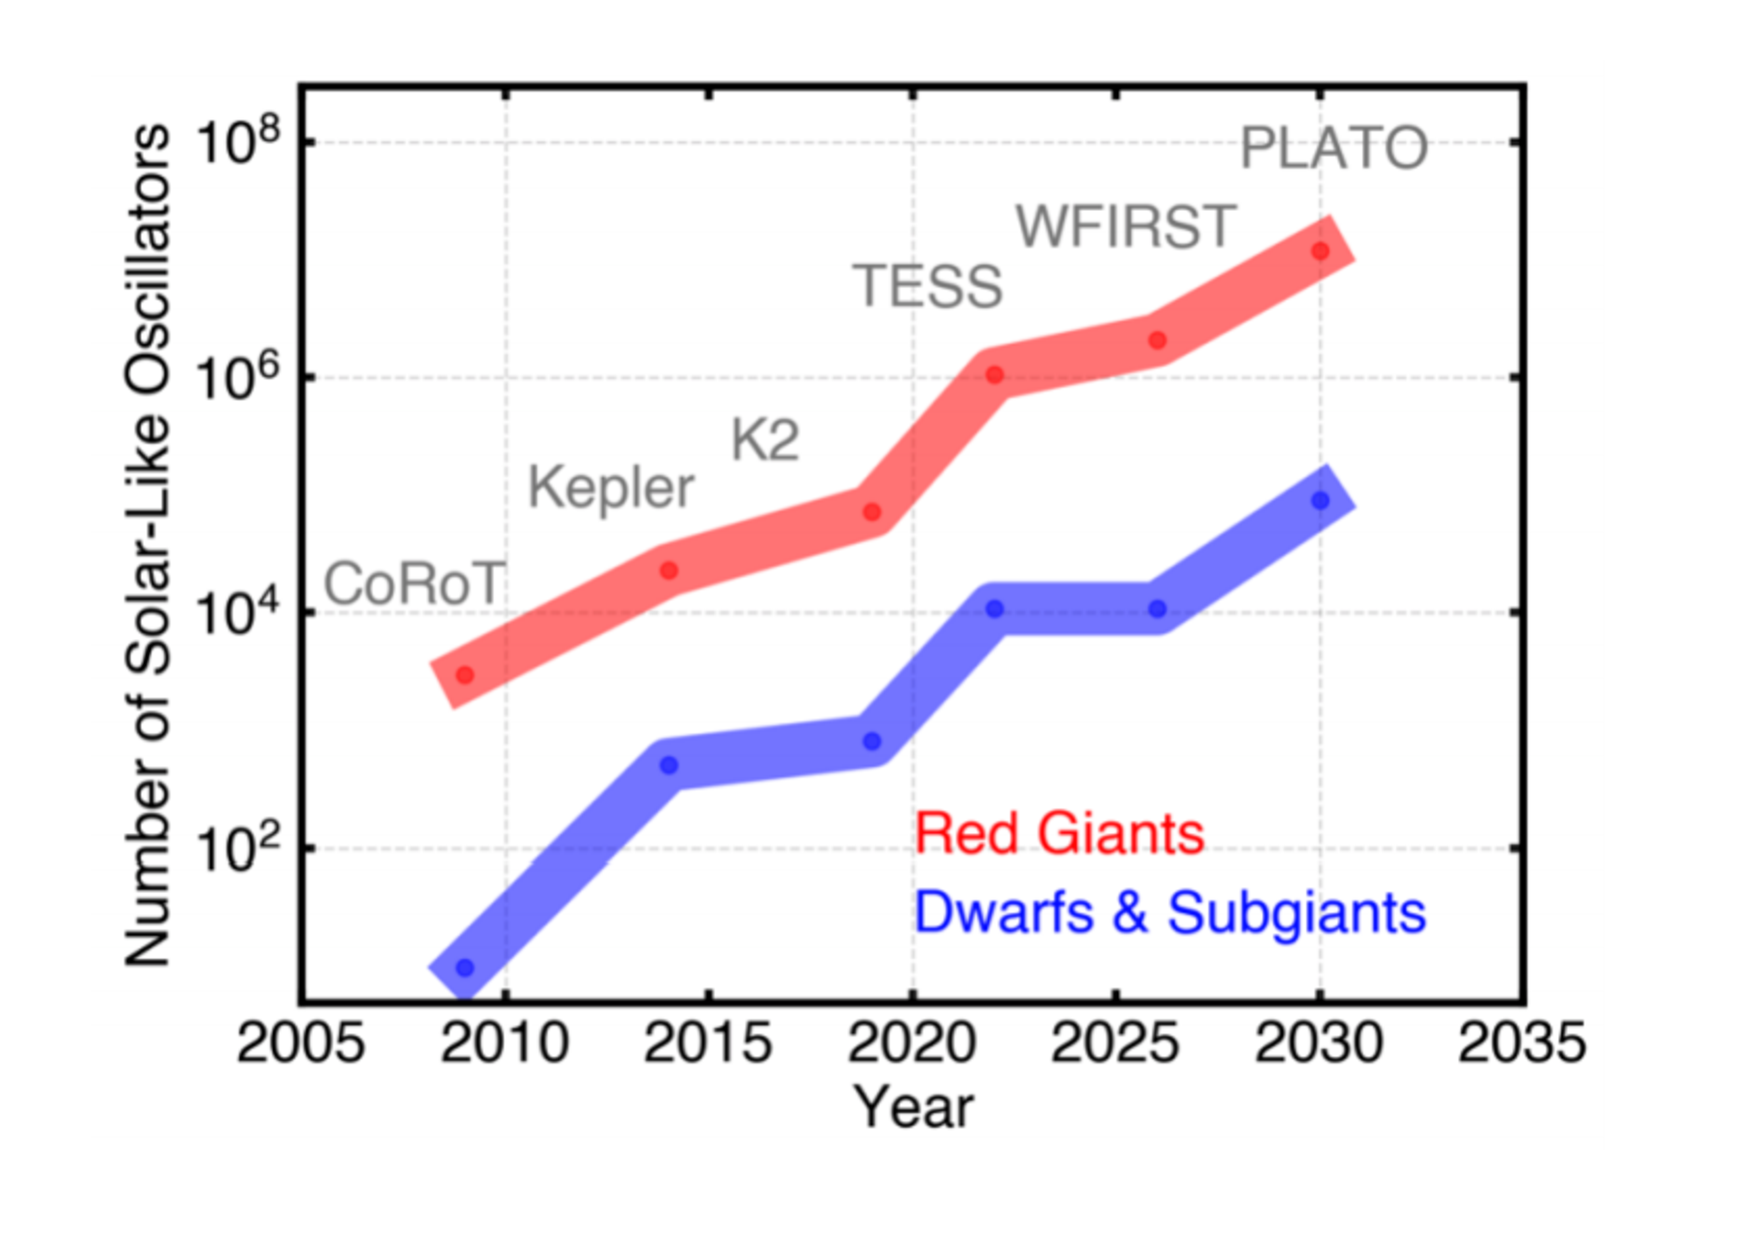
\includegraphics[width=0.8\textwidth]{Figures/number_of_stellar_ages.pdf}
    \caption[Expected yield of solar--like oscillators with current and future telescopes]{Yield of solar--like oscillators discovered and expected to be discovered by space--based telescopes, separated into dwarfs and subgiants, and red giants. Image credit: \citet{Huber_etal_2019_white_paper}}
    \label{fig:number_of_stellar_ages}
\end{figure}

The work presented in this thesis is just the beginning for utilising asteroseismic ages to calibrate the age--activity--rotation relationship. The era of large samples of stellar ages is yet to come, as demonstrated in Figure \ref{fig:number_of_stellar_ages}, with a significant increase in the number of stellar ages expected to be determined during the 2020's. Progress with \textit{TESS} is underway with the first \textit{TESS} detection of an exoplanet host with asteroseismic analysis published this year \citep{Huber_etal_2019}. Further progress will be made with the \textit{PLATO} mission \citep{Rauer_etal_2014}, which is being designed with the core science goal of determine planet radii and masses along with accurate ages for these systems, through asteroseismology. \textit{PLATO} is due to launch in 2026. As the number of stars with determined ages increases, future studies concerning the age--activity--rotation relationship will be able to shed more light on the exact nature of the relationship and build upon the work started in recent years including the work presented in this thesis.

